\documentclass[10pt,twocolumn,letterpaper]{article}

\usepackage{cvpr}
\usepackage{times}
\usepackage{epsfig}
\usepackage{graphicx}
\usepackage{amsmath}
\usepackage{amssymb}

% Include other packages here, before hyperref.

% If you comment hyperref and then uncomment it, you should delete
% egpaper.aux before re-running latex.  (Or just hit 'q' on the first latex
% run, let it finish, and you should be clear).
\usepackage[pagebackref=true,breaklinks=true,letterpaper=true,colorlinks,bookmarks=false]{hyperref}

% \cvprfinalcopy % *** Uncomment this line for the final submission

\def\cvprPaperID{****} % *** Enter the CVPR Paper ID here
\def\httilde{\mbox{\tt\raisebox{-.5ex}{\symbol{126}}}}

% Pages are numbered in submission mode, and unnumbered in camera-ready
\ifcvprfinal\pagestyle{empty}\fi
\begin{document}

%%%%%%%%% TITLE
\title{Bayesian Fracture Modeling from Video Evidence}

\author{Simon Swenson\\
University of Arizona\\
{\tt\small simonswenson@email.arizona.edu}
% For a paper whose authors are all at the same institution,
% omit the following lines up until the closing ``}''.
% Additional authors and addresses can be added with ``\and'',
% just like the second author.
% To save space, use either the email address or home page, not both
\and
Kobus Barnard\\
University of Arizona\\
{\tt\small kobus@cs.arizona.edu}
\and
Josh Levine\\
University of Arizona\\
{\tt\small josh@email.arizona.edu}
}

\maketitle
%\thispagestyle{empty}

%%%%%%%%% ABSTRACT
\begin{abstract}
    Despite previous research in modeling physical properties from video 
    evidence, no work for modeling the physical properties of rigid objects, 
    such as pottery and logs,
    as they undergo fracture exists, to our knowledge. We note several key 
    elements that should be included in any such physical model of fracture, 
    namely, that the modeling is in 3-d, and that the following elements are 
    included: (1) the time of fracture, (2) the geometry of the initial object 
    and subsequent fragments, including the number of fragments, (3) the 
    physical properties of the fragments, including position and momentum, and 
    (4) collision between objects. To 
    this end, we propose a probablistic graphical model that includes priors 
    of the laws of physics to infer these hidden 
    variables from pre-processed (TODO what kind?) image data, using (TODO) 
    inference technique. To evaluate this model and inference technique, we 
    use the (TODO) method on the (TODO) dataset. 
    Our initial experiments show that (TODO).
\end{abstract}

%%%%%%%%% BODY TEXT
\section{Introduction}

Fracture events are of interest to many clients. Departments of 
transporation are responsible for the quick response to and recovery from 
quickly changing roadside conditions. For mountainous roads, this can include 
rock slides and 
the collapse of rock cliffs onto the roadway. Another class of organizations, 
mining companies, require prediction and modeling of the geology for possible 
failures as they extract 
minerals from the earth, changing the landscape in the process. Third, 
structural collapses such as dam failures 
can be catostrophic, and civil engineers would benefit from 
an ability to model and predict such collapses.

Any insight provided to these clients is helpful, and, to do so, we must model 
the fracture event, including its underlying physical properties. While 
it is impossible to perfectly model physics with current computing capabilities, 
and it would be even more difficult to find a matching physical simulation given 
video evidence, we identify several key properties that a physical model for 
fracture should include and several simplifying assumptions to make the model 
more manageable. First, for a fracture to have occurred in the first 
place, a time span over which it occurs is required. For rigid objects which 
shatter very quickly, 
as opposed to flexible objects that fail in a ductile way, this time 
span becomes very close to a single point in time. Thus, we make the 
simplifying assumption that the fracture occurs at a single point in time.

Second, the geometry of the objects should be included. For a fracture event, 
this means that an object with one geometry becomes many objects, a partition 
of the geometry of the original object. In theory, this partition could be 
arbitrary, but we make the simplifying assumption that partition can be 
determined by a recursive binary partition along boundaries that are roughly 
planar. Furthermore, we assume that no extremely small fragments, i.e., dust, 
exist. In reality, the existence of such small dust fragments are negligible, in 
light of the much larger fragments.

Third, the physical properties of the objects should be included. 
This includes positional properties, namely, the position and angle of the 
original object and each fragment's center-of-mass and associated velocities, 
for each video frame. Here, we assume that the initial object is 
stationary. This simplifies the model in that, before the fracture, the only 
object that is moving is the object causing the fracture, whereas, in the 
general case, one or more of (1) the object which is fractured and (2) the 
object which is causing the fracture, may be moving. When the fracture happens, 
finding out the new positions and velocities of all the new fragments requires 
an additional physical property: the energy which was added by the object which 
caused the fracture. Aside from this added energy, we assume conservation of 
energy, and thus momentum, for the fragments.
After the fracture has 
happened, distance and velocity values should update deterministically from 
the physical laws of motion. In practice, though, this is unteneble. Therefore, 
we assume that probablistic updates occur at discrete time points. These 
probablistic updates can still incorporate physical priors (as the 
mode of the probablistic update).

Fourth, collision between objects should be modeled. In the general case, and 
especially with geometry that includes concavities, calculations for collision 
detection can be costly. If we begin with convex geometry or geometry 
that is decomposed into a partition of convex geometry, the assumption of planar 
fracture ensures that the only kind of geometry that we deal with is convex. 
This simplifying assumption makes 
collision detection much simpler, which also makes our machine learning approach 
more tenable.

\section{Problem Statement}

In the context of video evidence, the requirements of the physical fracture 
model outlined above require solving several 
difficult tasks. First, the time of fracture must be identified from the video 
sequence evidence. Initially, this may not 
seem like that difficult of a task, and, indeed, it is certainly not the most 
difficult problem. However, this can be complicated due to other movement in the 
scene, namely movement of the object causing the fracture.

Second, the number of fragments after the fracture event should be found, 
to model their geometry and motion accurately. This is made 
difficult due to the nature of fracture of rigid objects: Fractures typically 
occur quickly, between camera frames. In other words, the single object becomes 
many in the span of a frame. Occlusion also complicates this task, as some of 
the fragments could be occluded by others.

Another task is identifying the fragments’ positions in the frame. The objects 
we are dealing with could be moving very fast and be 
very small. Even in simple video sequences with a stark difference in value 
between the object and the background, existing segmentation techniques may fail 
to segment the fragments from each other. Further complicating 
things, motion blur 
means that a single frame could provide evidence for a range of positions for 
each fragment. Even examining the frame sequences in their entirety, using 
motion of the image patches as evidence, traditional techniques for finding motion of 
image patches of sequences, like optical flow, have 
difficulty with such fast movement of such small objects.

In addition, physical modeling requires a notion of the geometry of the object. Typical 
surface reconstruction techniques, like structure from motion, require multiple 
views to recover a point cloud that represents the geometry of the scene, and, 
even then, further processing is required to obtain an object volume.

Last, in addition to geometry, properties like position and momentum in 
3-d require a notion of pysics, to connect the evidence from the previous tasks 
to the physical properties. However, deterministic physics simulation suffers 
from chaos theory. Small changes in the initial conditions produce wildly 
different outputs.

\subsection{Background}

Our strategy for tackling this problem has been to start with simpler versions 
of the problem and work our way up from there. It is important to identify three 
different dimensionalities that can each be moved up or down to complicate or 
simplify the model: (1) the dimensionality of the world, (2) the 
dimensionality of the object being fractured, and (3) the dimensionality of the 
space onto which the world will be projected.

For fracture of arbitrary, real objects in the real world, both (1) and (2) 
would be 3-d. However, it is also important to note that certain real-world 
objects like sheets of glass can be represented in lower dimensions. Our 
simplifications have focused on lower dimesionality along (1) and (2), while 
leaving (3) 2-d (images). So far, we have only worked in 2-d for (1). However, 
we have varied the dimensionality of the object.

We began with a 0-d object, which can be thought of as a single particle. This 
allowed us to perform position and velocity updates according to initial 
position and velocity random variables and a fixed gravitational constant. 
From there, we moved onto a 1-d 
object, a path in 2-d space, with the restriction that the path was straight. 
The existing physics updates for the 0-d model were 
incorporated as the stick's center of mass. Additionally, we added angle 
and angular velocity (and corresponding random variables) to the model. From 
here, we added fracture to the model, 
beginning with a single fracture. At this point, we allowed the fracture to occur at 
an arbitrary frame of the video, which meant that the model had changing 
dimensionality. We shortly added a binary fracture model, in which a single 
stick splits into at most two sticks in a single frame of the video and that the 
stick ancestry could be represented by a full binary tree. The 
corresponding Bayes net can be seen in the nearby figure. A model (with 2-d blocks) 
that is very similar to the model in the figure will later be explained.

\begin{figure}[t]
\begin{center}
   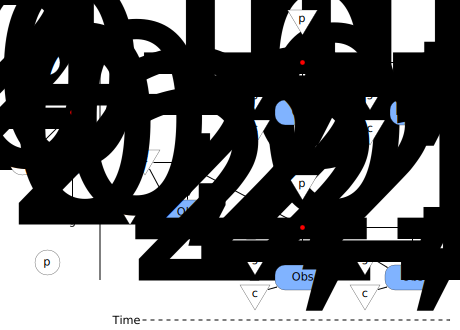
\includegraphics[width=0.8\linewidth]{figs/2d-stick-net-20190930.png}
\end{center}
   \caption{The Bayesian Network for the 2-d world, 1-d object (stick) model. Here, 
        there are three video frames and three objects: one parent object and 
        two fragments. The fracture time has already sampled from 
        a discrete distribution: $FT_0 = 2$. A very similar model, the 
        2-d block model, is explained later.}
\label{fig:long}
\label{fig:onecol}
\end{figure}

From here, some preliminary work was done to explore potential 
inference techniques that we could use. We devised an experiment using 
Metropolis-Hastings random walk to infer the continuous variables while leaving the discrete 
variable, the time of fracture, fixed at its known value. In order to ensure 
that the inference worked at all, we devised a noise model that ensured that 
the observations for any data set had support over the space of priors. To do 
so, we added IID noise to each observed end point in the image space. 
Unfortunately, our results using Metropolis-Hastings were initially poor. We ran inference with 
chain lengths of 100,000. We had to use narrow standard deviations for the 
proposal distributions to achieve a reasonable acceptance rate, but this also 
meant that the chains were slow to converge and were prone to getting caught 
in local optima.

\subsection{2-d Block, 2-d World Model}

At this time, we moved onto a model with 2-d objects to better approximate the 
data sets that we were interested in at the time, firewood cutting videos. We 
still maintained a 2-d world. While this model may seem to 
complicate things in comparison to the 1-d stick model, several assumptions were made to 
simplify the 2-d objects. We enforced  
that the objects were rectangles (blocks), oriented orthogonally the world's standard 
basis. We also took a step back and simplified the fracture event. We  
enforced that the block did not move until the fracture happened. This 
allowed us to collapse all frames before the fracture to a single frame. In 
other words, in this model, there is no change of dimensionality. We also 
incorporated the conservation of momentum and angular momentum into this model, 
enforcing that, since the object is initially stationary, the sum of the momenta 
from the two fragments is 0.

We explain this model in detail. A large portion of the network is dedicated to physical modeling, but the model 
must also incorporate the video sequence. This includes a camera as well as the 
pre-processed data from images that that camera produced. First, we define 
several values that are given as hyper-parameters:

\begin{itemize}
    \item $I_w$: width of the images
    \item $I_h$: height of the images
    \item $M$: number of images
    \item $C_{fps}$: frames per second of the camera
\end{itemize}

and the calculated image aspect ratio and gravity constant:

\begin{align*}
    I_{ar} =&  \frac{I_w}{I_h} \\
       a_y =& -\frac{9.8}{(C_{fps})^2}
\end{align*}

Next, we sample a camera. For a 2-d embedding space, this is as simple as 
sampling the top of the camera, in world units -- meters -- and calculating the 
right boundary from that and the image aspect ratio:

\begin{align*}
     C_l =& 0 \\
     C_b =& 0 \\
    C_t \sim& TruncNormal(\mu=3,\sigma=1,low=0,high=\infty) \\
     C_r =& C_t \times I_{ar}
\end{align*}

From these values, we calculate the meters per pixel and define a linear 
transformation from world coordinates to image pixels:

\begin{align*}
    \frac{m}{pix} =& \frac{C_t - C_b}{I_h} \\
          C_{mat} =& \begin{bmatrix}
                        0 & -\frac{pix}{m} &  \frac{C_t \times pix}{m} \\
            \frac{pix}{m} &              0 & -\frac{C_l \times pix}{m} \\
                        0 &              0 &                         1
        \end{bmatrix}
\end{align*}

We can also sample the block dimensions and positions in terms of world 
coordinates, meters, using priors on the shapes and sizes of logs that are used 
for firewood. We use the notation 
$S_{n,m}$, a record over fragment ID $N$ 
and timestamp $M$, each indexed from 0, which represents the state of that 
fragment's center of mass at that timestamp. Each such record contains both position, 
$q$, velocity, $v$, angle, $\Theta$, and angular velocity, $\omega$ of which 
non-angular values are indexed by dimension, ($x, y$). For 
example, $S_{3,4}.q_y$ indicates the y position for 
the third fragment at the fourth frame. $L_n$ is a record representing the geometry for 
block $n$, including $w, h$ as well as a $g$, calculated geometry, a 
sequence of points in 2-d homogeneous coordinates for the block, in a space 
relative to the block's center of mass, and $v$, the volume of the block.

\begin{align*}
       S_{0,0}.q_x \sim& Normal(\mu=\frac{C_l + C_r}{2},\sigma=\frac{C_r - C_l}{16}) \\
       S_{0,0}.q_y \sim& Normal(\mu=\frac{C_t + C_b}{2},\sigma=\frac{C_t - C_b}{16}) \\
          S_{0,0}.v =& \overrightarrow{0} \\
     S_{0,0}.\Theta =& 0 \\
     S_{0,0}.\omega =& 0 \\
             L_0.w \sim& TruncNormal(\mu=0.2,\sigma=0.075, \\ 
                       & \qquad low=0,high=\infty) \\
             L_0.h \sim& TruncNormal(\mu=0.3,\sigma=0.2, \\ 
                       & \qquad low=0,high=\infty) \\
              L_n.g =& \begin{bmatrix}
                  \frac{-L_n.w}{2} & \frac{L_n.w}{2} &  \frac{L_n.w}{2} & \frac{-L_n.w}{2} \\
                   \frac{L_n.h}{2} & \frac{L_n.h}{2} & \frac{-L_n.h}{2} & \frac{-L_n.h}{2} \\
                                 1 &               1 &                1 &                1
              \end{bmatrix} \\
              L_n.v =& L_n.w \times L_n.h
\end{align*}

We move onto the fracture event, itself. Since we assume the initial block is 
stationary, we model the fracture event as always happening at $m = 1$. Currently, we do 
not model any additional energy added to the system. However, we do sample a 
momentum and angular momentum for the left block (block 1), and, using 
conservation of momentum, determine the corresponding momenta of the right block 
(block 2). For objects on a platform, we assume that there is no y momentum 
added. We also sample the fracture location for the vertically-oriented fracture 
plane:

\begin{align*}
    mom_{1,x} \sim& TruncNormal(\mu=0, \sigma=0.05, \\
                  & \qquad low=-\infty, high=0) \\
     mom_{2,x} =& -mom_{1,x} \\
      angmom_1 \sim& TruncNormal(\mu=0, \sigma=0.2, \\ 
                   & \qquad low=0, high=\infty) \\
      angmom_2 =& -angmom_1 \\
         FL_0 \sim& TruncNormal(\mu=\frac{L_0.w}{2},\sigma=\frac{L_0.w}{4}, \\
                  & \qquad low=0,high=L_0.w) \\
         L_1.w =& FL_0 \\
         L_2.w =& L_0.w - FL_0 \\
         L_1.h =& L_2.h = L_0.h
\end{align*}

After sampling the fracture variables, we calculate the initial states of the 
new blocks' centers of mass and the new blocks' geometry. This is straightforward. We 
use the volume (area in 2-d) of the blocks and the momenta to calculate the 
added velocities. From here, we use Euler's method to determinstically update 
each block's state variables:

\begin{align*}
       S_{n,m}.q_x =& S_{n,(m-1)}.q_x + S_{n,(m-1)}.v_x \\
       S_{n,m}.q_y =& S_{n,(m-1)}.q_y + S_{n,(m-1)}.v_y \\
       S_{n,m}.v_x =& S_{n,(m-1)}.v_x \\
       S_{n,m}.v_y =& S_{n,(m-1)}.v_y + a_y \\
    S_{n,m}.\Theta =& S_{n,(m-1)}.\Theta + S_{n,(m-1)}.\omega \\
    S_{n,m}.\omega =& S_{n,(m-1)}.\omega
\end{align*}

From here, we project the points of each block into world coordinates via a 
transformation in terms of the position and angle of that block at that 
frame. Then, we project those coordinates into image coordinates using the 
camera matrix above, call these points $Act_{n,m,o,p}$, where $n, m$ are 
indexed as above and $o, p$ are point index and dimension 
index, respectively. Finally, we add some IID noise to those points:

\begin{align*}
    Obs_{n,m,o,p} \sim& Normal(\mu=Act_{n,m,o,p},\sigma=\frac{\sqrt{I_w \times I_h}}{512})
\end{align*}

We are currently exploring Metropolis-Hastings over this model. While experiments 
have been run, I need to do some data wrangling to reach any meaningful 
conclusions. After using multiple chains and increasing the chain length to 
1,000,000, some of the results look promising in isolation, but it remains to be 
seen whether it is an adequate technique for this model in general.

\section{Proposed Approach}

\subsection{Model}

There are seveal roadblocks that need to be overcome to convert the simplified 
models above so that they can be used to model real-world fracture events with 
real observation image sequences.

First, the camera will need to be changed when the world is changed to 3-d. 
However, existing work from the IVILAB has used a 3-parameter 
camera.\cite{Brau_2013_ICCV} This has been adquate to model the vast majority of stationary cameras,
so I am planning to use the 3-parameter camera model.

To convert the object model to 3-d, our object priors must change. The needed 
priors depend on the types of data that we are interested in. For the firewood 
cutting videos, we might model the blocks as vertically-oriented cylinders in 
$R^3$. For pottery, the objects are essentialy 2-d curves which are revolved 
around the z axis.

The fracture model will also need to be changed to reflect the real world. As with 
the object priors, fracture will depend on the types of data and fractures 
that we are interested in modeling. For firewood 
cutting, The fracture location could be modeled with a vertically-oriented 
plane. Energy added from the axe swing would also need to be incorporated. 
In addition, the corresponding added momenta must be oriented away from the 
fracture plane so that the fragments will move apart from each other.

Another important addition is collision. By only considering convex objects 
(as seen in "Introduction" above) collision can be easily calculated, so I am 
not too concerned with incorporating collision.

Finally, the model should be changed such that all deterministic quantities 
become probablistic "spring" variables. This should make inference more tenable.

\subsection{Inference}

A model specification alone does not solve the computer vision problem in its 
entirety. Efficient inference over the model is also necessary. Despite some 
preliminary, isolated Metropolis-Hastings random walk results that seem to work 
adequately with the 2-d block model, several 
differences between this simple model and the proposed 3-d model make us 
believe that random walk Metropolis-Hastings will cease to be a reasonable inference 
technique. First, incorporating spring constraints between each frame in the 
video, for each physical property, for each fragment, explodes the 
dimensionality of the space of random variables. It has been shown that 
Metropolis-Hastings suffers from the curse of dimensionality, with very small 
proposal standard deviations needed to achieve a reasonable sample acceptance rate 
in high-demensional spaces.\cite{Neal2011MCMCUH} However, the algorithm is 
more prone to getting "stuck" in local minima with narrower standard deviations.

One alternative class of inference techniques is variational 
inference. However, variation inference requires conjugate priors over all 
variables, which our model does not have. Thus, variational inference will not 
work.

Gibbs sampling is an oft-used sampling technique to more efficiently explore the 
posterior space by isolating and resampling each variable from its 
full conditional probability. However, Gibbs sampling requires these full 
conditional distributions. I think the model is too complicated to have 
tractible full conditionals.

Another straightforward improvement to Metropolis-Hastings is HMC. However, our 
model also has some constraints that introduce discontinuities into the 
posterior distribution. HMC has been shown to perform poorly when the sample 
meets a discontinuous boundary, and we most certainly have such constraints. 
(See the "TruncNormal" distributions in the 2-d block model.) If the
constraints occur where the posterior already had very low probability density,  
the samples may never meet a discontinuity in practice. In this case, we may 
hand-wave this problem away. However, the momenta variables above have 
constraints at the means of their distributions. Thus, we might have to turn to 
another solution, one outlined by.\cite{NIPS2015_5801} If we 
cannot find a way to 
get HMC to work, we will have to explore other inference techniques.

Our model is also changing dimensionality, making inference yet more 
difficult. One option for dealing with this is reversible jump MCMC. 
Alternatively, Kobus has 
suggested that I attempt to ignore the changing dimensionalty problem. I have 
to follow up with him about this, but it sounds like I may just be able to setup 
the model in such a way that I define a maximum number of supported fragments 
and then simply flag each fragment as either enabled or disabled.

In addition to the model definition and inference over that model, the kind of 
preprocessing evidence that we want to use with that model must be determined. 
We have already tracked down optical flow as a potential source of data, but 
I do not think optical flow, alone, will be enough to get good results. Other 
options I should explore include segmentation and shape from shading. Shape 
from shading may be extremely valuable for pottery videos, but this also 
requires a known light source. Image feature points, like those from SIFT, 
may also be helpful data for the model, specifically in identifying the fragments 
and their orientations in the image plane.

\section{Related Work}

\subsection{Tracking}

While we frame our proposal in terms of physical modeling, there is some overlap 
between our goal and tracking. Tracking is a broad field of research, and many 
techniques exist which produce a variety of object representations in the image 
plane. The most prominent object representation in use is bounding boxes, but Yilmaz 
et al.\cite{Yilmaz:2006:OTS:1177352.1177355} note two object representations that are closer to the 
output of our model: primitive geometric shapes, as used in \cite{Comaniciu2003} and object silhouette, 
as used in \cite{YILMAZ2003623}.

% TODO how do these relate to our problem? Will they fail?

Statistical methods have been employed for tracking in \cite{4767755} \cite{BarShalom1990} \cite{317728} \cite{Brau_2013_ICCV}.
Brau et al.\cite{Brau_2013_ICCV} use a generative, graphical model which models people as cylinders 
as they move within the frame and the images from the perpective of a 
simplified, three parameter camera.

Deep learning has been leveraged extensively for tracking problems.\cite{LI2018323} 
Deep learning approaches generally rely extensively on labeled data. This means that the data sets 
available and the labels provided affect the kinds of outputs that such deep 
learning approaches can produce. Importantly, the vast majority of deep learning 
approaches produce bounding box representations of the objects. Instead, we seek 
to represent the objects as 3-d geometry.

Overall, we found no existing tracking techniques designed to handle a single 
object splitting into multiple objects.

\subsection{Physical Modeling}

Some work has been done in using video evidence to infer various physical 
properties of objects, from position, to velocity, to mass, to more complicated 
properties. In “Physics 101: Learning Physical Object Properties from Unlabeled 
Videos,” 2016, Wu et al. used a convolutional neural network in conjunction with 
hard-coded physics equations to infer a myriad of physical properties, from mass 
to coefficients of friction, in a variety of scenarios, from ramps to springs to 
a liquid scenario.

In “What Players do with the Ball: A Physically Constrained Interaction Modeling,” 
2016, Maksai et al. use probabilistic graphical modeling to introduce physical 
constraints into the task of tracking in sports videos, made difficult due to 
the balls’ small size and quick speed.

Many other papers exist in this domain, but, in our literature review thus far, 
we have seen none tackle the task of inferring physical properties in a fracture 
scenario.

{\small
\bibliographystyle{ieee_fullname}
\bibliography{egbib}
}

\end{document}
